\chapter{{\fontsize{14pt}{21pt}\selectfont\MakeUppercase{Предметная область и технологии}}}
\label{cha:analysis}

\section{Исследование предметной области}

На начальном этапе разработки рассмотрен практический сценарий пользователя, который стремится планировать рацион системно: подбирать рецепты, учитывать ограничения по питанию, формировать меню на период и получать список покупок. Анализ существующих пользовательских сценариев показывает, что эти действия часто распределены между несколькими сервисами: кулинарными порталами, приложениями учета калорий и отдельными инструментами ведения заметок.

При таком подходе возникают повторяющиеся операционные трудности: дублирование данных, ручной перенос информации между сервисами, отсутствие единой модели пользовательских предпочтений и ограничений, а также разрыв между этапом выбора блюда и этапом практического исполнения плана (покупка продуктов). В результате возрастает время на планирование и снижается управляемость процесса в долгосрочном периоде.

Предварительный обзор существующих решений показывает, что на рынке присутствуют как кулинарные платформы, так и специализированные сервисы учета питания, однако пользовательский сценарий часто остается разорванным между несколькими инструментами \cite{nutristeppe_diaries_2026,institutfitnesa_apps_2026,sportmaster_apps_2026}. Детальный сравнительный анализ конкурентов и аналогов приведен в разделе~1.4.

\section{Определение целевой аудитории}

Целевая аудитория разрабатываемого веб-приложения включает группы пользователей, объединенные общей потребностью в системном управлении питанием, но различающиеся по сценариям использования.

Основная пользовательская аудитория

К основной аудитории относятся пользователи, планирующие рацион в соответствии с персональными целями:
\begin{compactlist}
  \item снижение массы тела, поддержание формы или набор массы;
  \item учет персональных ограничений в питании;
  \item ускорение ежедневного планирования меню;
  \item получение рекомендаций по выбору блюд и структуры рациона.
\end{compactlist}

Ключевые требования этой группы:
\begin{compactlist}
  \item персонализация рекомендаций и фильтрации;
  \item визуально понятное планирование по дням и приемам пищи;
  \item контроль КБЖУ и состава блюд \cite{sektascience_bzhu_2026};
  \item формирование практического списка покупок на основе выбранного меню.
\end{compactlist}

Авторы пользовательского контента

В данную группу входят пользователи, которые создают рецепты, публикуют планы питания и оставляют отзывы.

Для этой категории критичны:
\begin{compactlist}
  \item удобные формы публикации и редактирования материалов;
  \item прозрачность статусов модерации контента;
  \item получение обратной связи от других пользователей.
\end{compactlist}

Ролевые группы в системе

Ролевые группы описывают не целевую аудиторию, а модель разграничения прав доступа в программной системе.

Пользователь

Базовая роль, обеспечивающая работу с рецептами, планами питания, отзывами, избранным и списками покупок в рамках собственных данных.

Модератор

Роль контроля качества контента: проверка рецептов, отзывов и жалоб, принятие решений по модерации, корректировка публикаций в пределах регламента платформы.

Администратор

Роль расширенного системного управления: управление учетными записями и ролями, администрирование справочников, контроль устойчивости и безопасности функционирования платформы.

\section{Проектирование бизнес-процессов}

Бизнес-процесс представляет собой совокупность связанных активностей, преобразующих входные данные в результат, имеющий ценность для пользователя \cite{kirillina_bpm_2022}. Для формализации процессов в рамках проекта используется подход структурного анализа и проектирования SADT (Structured Analysis and Design Technique), в составе которого применяется семейство нотаций IDEF \cite{mindalev_idef_2016,sadt_intro_ross,idef0_fips_183}.

Краткая характеристика основных нотаций IDEF приведена в таблице~\ref{tab:idef-notations}.

\begin{table}[H]
\caption{Краткая характеристика нотаций IDEF}
\label{tab:idef-notations}
\small
\begin{tabularx}{\textwidth}{|p{0.16\textwidth}|p{0.30\textwidth}|X|}
\hline
\multicolumn{1}{|c|}{Нотация} & \multicolumn{1}{c|}{Назначение нотации} & \multicolumn{1}{c|}{Основные отражаемые объекты} \\ \hline
IDEF0 & Создание функциональной модели & Функции, входы/выходы, управляющие воздействия и механизмы выполнения процессов. \\ \hline
IDEF1 & Построение информационной модели & Информационные потоки и структура данных предметной области. \\ \hline
IDEF1X & Построение реляционных структур & Сущности, атрибуты и связи между сущностями в терминах реляционной модели. \\ \hline
IDEF3 & Документирование сценариев выполнения процессов & Последовательность операций и варианты прохождения процесса. \\ \hline
IDEF5 & Онтологическое описание сложных систем & Классы объектов, отношения, ограничения и изменения состояния. \\ \hline
\end{tabularx}
\normalsize
\end{table}

Для проектирования ключевого процесса <<Составление плана питания пользователем>> в проекте использована нотация IDEF0, а для описания межролевого взаимодействия --- BPMN 2.0 \cite{mindalev_idef_2016,zueva_bpmn_2021,bpmn_spec_2014}.

Нотация BPMN 2.0 поддерживает несколько типов представлений: оркестровка (один пул с внутренним потоком управления), диаграмма взаимодействия (несколько пулов и обмен сообщениями), хореография и схема диалога \cite{zueva_bpmn_2021,bpmn_spec_2014}. В рамках FoodPlanner практическую ценность для описания пользовательских и системных сценариев имеют оркестровка и диаграмма взаимодействия.

Диаграмма вариантов использования на \hyperref[fig:uml-users]{рисунке~\ref*{fig:uml-users}} показывает распределение сценариев между ролями системы.

\begin{figure}[H]
  \centering
  
\includegraphics[width=0.95\textwidth]{UML.png}
  \caption{UML-диаграмма пользователей}
  \label{fig:uml-users}
\end{figure}

Неавторизованный пользователь (гость) имеет доступ к просмотру каталога рецептов и регистрации в системе. После прохождения регистрации пользователь получает возможность авторизации и перехода к персональным сценариям.

Авторизованный пользователь, помимо просмотра каталога, может редактировать профиль, указывать предпочтения, создавать и редактировать собственные рецепты, собирать планы питания, формировать список покупок, оставлять оценки и отзывы, а также использовать ИИ-ассистента и просматривать персональную аналитику.

Администратор обеспечивает управленческие и контрольные функции: управление пользователями и ролями, администрирование справочников, контроль жалоб и контроль корректности модерационных процессов.

Процесс взаимодействия пользователя с планом питания представлен BPMN-диаграммой (\hyperref[fig:bpmn-plan-interaction]{рисунок~\ref*{fig:bpmn-plan-interaction}}).

\begin{figure}[H]
  \centering
  \IfFileExists{images/bpmn-plan-interaction.png}{
    
\includegraphics[angle=90,width=\textwidth,height=0.90\textheight,keepaspectratio]{bpmn-plan-interaction.png}
  }{
    \fbox{\parbox{0.9\textwidth}{\centering Место для рисунка BPMN\\
    Файл: \texttt{Report/images/bpmn-plan-interaction.png}}}
  }
  \caption{BPMN-диаграмма процесса взаимодействия пользователя с планом питания}
  \label{fig:bpmn-plan-interaction}
\end{figure}

Алгоритм составления плана питания пользователем приведен на \hyperref[fig:plan-creation-process]{рисунке~\ref*{fig:plan-creation-process}}.

\begin{figure}[H]
  \centering
  \IfFileExists{images/plan-creation-process.png}{
    
\includegraphics[width=\textwidth,height=0.88\textheight,keepaspectratio]{plan-creation-process.png}
  }{
    \fbox{\parbox{0.9\textwidth}{\centering Место для рисунка процесса\\
    Файл: \texttt{Report/images/plan-creation-process.png}}}
  }
  \caption{Процесс создания плана питания}
  \label{fig:plan-creation-process}
\end{figure}

\textbf{Взаимодействие пользователя с системой в рамках IDEF0}

Пользователь задает исходные условия: доступные продукты, цели питания, ограничения и предпочтения. Эти данные поступают на вход функциональной модели. Далее система последовательно выполняет анализ входных данных, подбор рецептов, формирование меню и генерацию списка покупок с расчетом пищевой ценности.

Контекстная диаграмма IDEF0 (уровень A-0)

На контекстном уровне система представлена единой функцией <<Планирование питания с учетом предпочтений пользователя>>. Входами являются данные о продуктах и целях питания; управлениями --- ограничения, предпочтения и нормативные параметры; механизмами --- веб-интерфейс, сервер приложений и база данных; выходами --- сформированное меню, список покупок и расчет пищевой ценности.

Декомпозиция IDEF0 (уровень A0)

Декомпозиция верхнего уровня включает четыре функциональных блока:
\begin{compactlist}
  \item анализ имеющихся продуктов;
  \item поиск подходящих рецептов;
  \item выбор оптимального меню на период;
  \item формирование списка недостающих покупок.
\end{compactlist}

Диаграммы IDEF0 и IDEF1 приведены на \hyperref[fig:idef0]{рисунке~\ref*{fig:idef0}} и \hyperref[fig:idef1]{рисунке~\ref*{fig:idef1}}.

\begin{figure}[H]
  \centering
  \IfFileExists{images/idef0.png}{
    
\includegraphics[angle=90,width=\textwidth,height=0.90\textheight,keepaspectratio]{idef0.png}
  }{
    \fbox{\parbox{0.9\textwidth}{\centering Место для диаграммы IDEF0\\
    Файл: \texttt{Report/images/idef0.png}}}
  }
  \caption{IDEF0-диаграмма бизнес-процесса}
  \label{fig:idef0}
\end{figure}

\begin{figure}[H]
  \centering
  \IfFileExists{images/idef1.png}{
    
\includegraphics[angle=90,width=\textwidth,height=0.90\textheight,keepaspectratio]{idef1.png}
  }{
    \fbox{\parbox{0.9\textwidth}{\centering Место для диаграммы IDEF1\\
    Файл: \texttt{Report/images/idef1.png}}}
  }
  \caption{IDEF1-диаграмма структуры данных}
  \label{fig:idef1}
\end{figure}

\section{Анализ аналогов и конкурентов}

Анализ аналогов и конкурентов выполнен для оценки уровня покрытия пользовательских потребностей, выявленных в предыдущих разделах: целостное планирование рациона, персонализация, учет ограничений, формирование списка покупок и поддержка модерации пользовательского контента. Дополнительно учтены обзорные публикации по приложениям и дневникам питания \cite{nutristeppe_diaries_2026,institutfitnesa_apps_2026,sportmaster_apps_2026}.

В качестве конкурентов и функциональных аналогов выбраны платформы, которые наиболее близки к сценарию FoodPlanner по пользовательским задачам: MenuBook, <<Еда>>, Ovkuse, <<Поварёнок>> и MyFitnessPal \cite{menubook2026,eda2026,ovkuse2026,povarenok2026,myfitnesspal2026}. Для оценки использовались следующие критерии: наличие конструктора плана питания, учет пищевых предпочтений, ИИ-помощник, доступность базового функционала без подписки, качество пользовательского интерфейса и наличие сообщества.

\begin{table}[H]
\caption{Сравнение конкурентов и аналогов}
\label{tab:analog-competitors}
\small
\begin{tabular}{|p{0.18\textwidth}|p{0.28\textwidth}|p{0.46\textwidth}|}
\hline
\multicolumn{1}{|c|}{Сервис} & \multicolumn{1}{c|}{Сильные стороны} & \multicolumn{1}{c|}{Ограничения для целевого сценария} \\ \hline
MenuBook & Праздничные сценарии меню, расчет ИМТ, базовые рекомендации, очень хорошее создание плана питания & Нет ИИ-ассистента; значимая часть сценариев платная; нет полноценного подбора по предпочтениям. \\ \hline
Еда (Rambler) & Сильный визуал, модерация рецептов, развитый контентный раздел & Нет конструктора плана питания, слабая персонализация по ограничениям, нет ИИ-ассистента. \\ \hline
Ovkuse & Большая рецептная база, активное сообщество, есть ИИ-ассистент & Много полезных функций доступно только по подписке; нет полноценного конструктора длительного плана питания. \\ \hline
Поварёнок & Крупная база рецептов, БЖУ, дневники, Q\&A, посты и видео & Устаревший интерфейс; нет ИИ-помощника и нет конструктора плана питания в целевом формате. \\ \hline
MyFitnessPal & Сильный онбординг по целям, трекинг прогресса, дэшборды & Фокус на учете и фитнесе; нет ИИ и нет гибкого конструктора меню по дням и приемам пищи. \\ \hline
\end{tabular}
\normalsize
\end{table}

MenuBook \cite{menubook2026} демонстрирует сильный сценарий подготовки меню под конкретный формат питания: пользователь может собирать меню, в том числе для специальных и праздничных случаев, а также получать базовые рекомендации и расчет индекса массы тела. Интерфейс сервиса ориентирован на быстрый переход к готовым сценариям, что упрощает вход для широкой аудитории. Вместе с тем платформа не предлагает встроенного ИИ-ассистента и не закрывает полноценный сценарий персонализации по ограничениям и предпочтениям пользователя. Интерфейс платформы MenuBook представлен на рисунке~\ref{fig:competitor-menubook}.

\begin{figure}[H]
  \centering
  \IfFileExists{images/competitor-menubook.png}{
    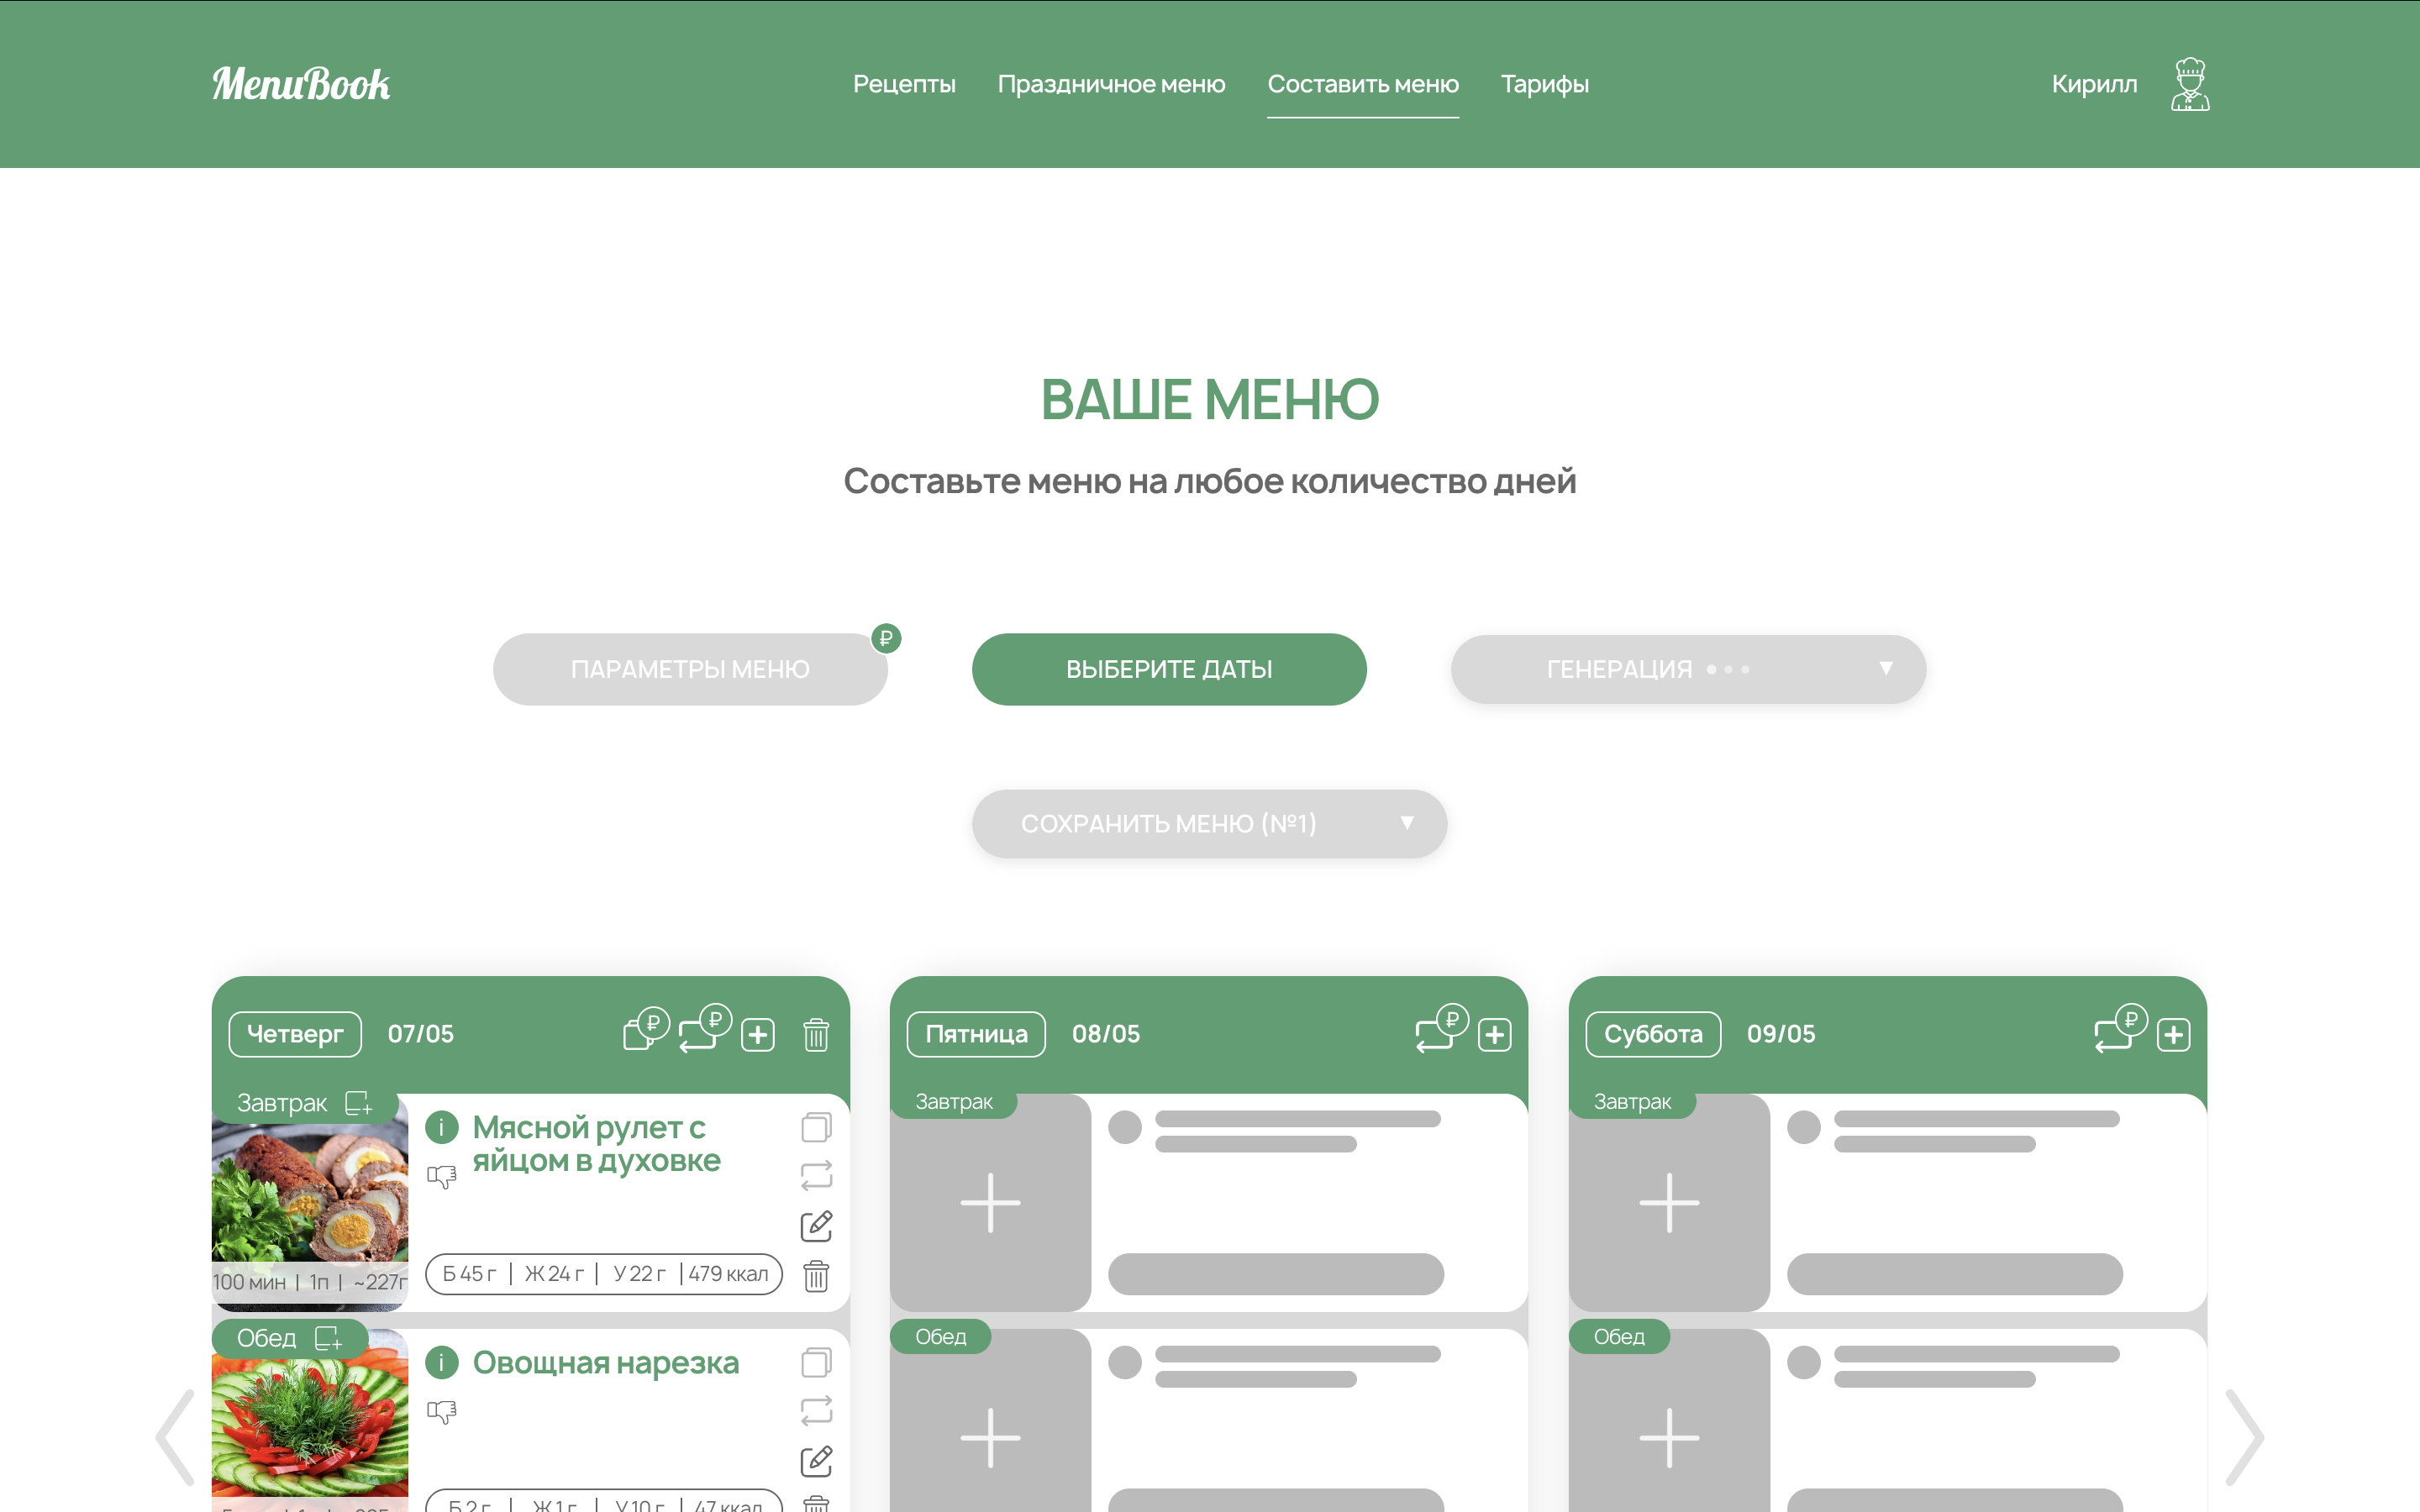
\includegraphics[width=\textwidth,height=0.82\textheight,keepaspectratio]{images/competitor-menubook.png}
  }{
    \fbox{\parbox{0.92\textwidth}{\centering Файл скриншота не найден: \texttt{images/competitor-menubook.png}}}
  }
  \caption{Интерфейс платформы MenuBook}
  \label{fig:competitor-menubook}
\end{figure}

Платформа <<Еда>> \cite{eda2026} показывает высокий уровень контентного качества и редакционного сопровождения: пользователь получает широкий выбор рецептов, статей и тематических подборок с удобной навигацией. Важным плюсом является зрелая контентная экосистема и стабильные пользовательские сценарии входа, что повышает удобство ежедневного использования. Однако основной фокус сервиса остается информационно-рецептурным, а не планировочным: отсутствует конструктор рациона и выраженная персонализация по пищевым ограничениям. Интерфейс платформы <<Еда>> представлен на рисунке~\ref{fig:competitor-eda-rambler}.

\begin{figure}[H]
  \centering
  \IfFileExists{images/competitor-eda-rambler.png}{
    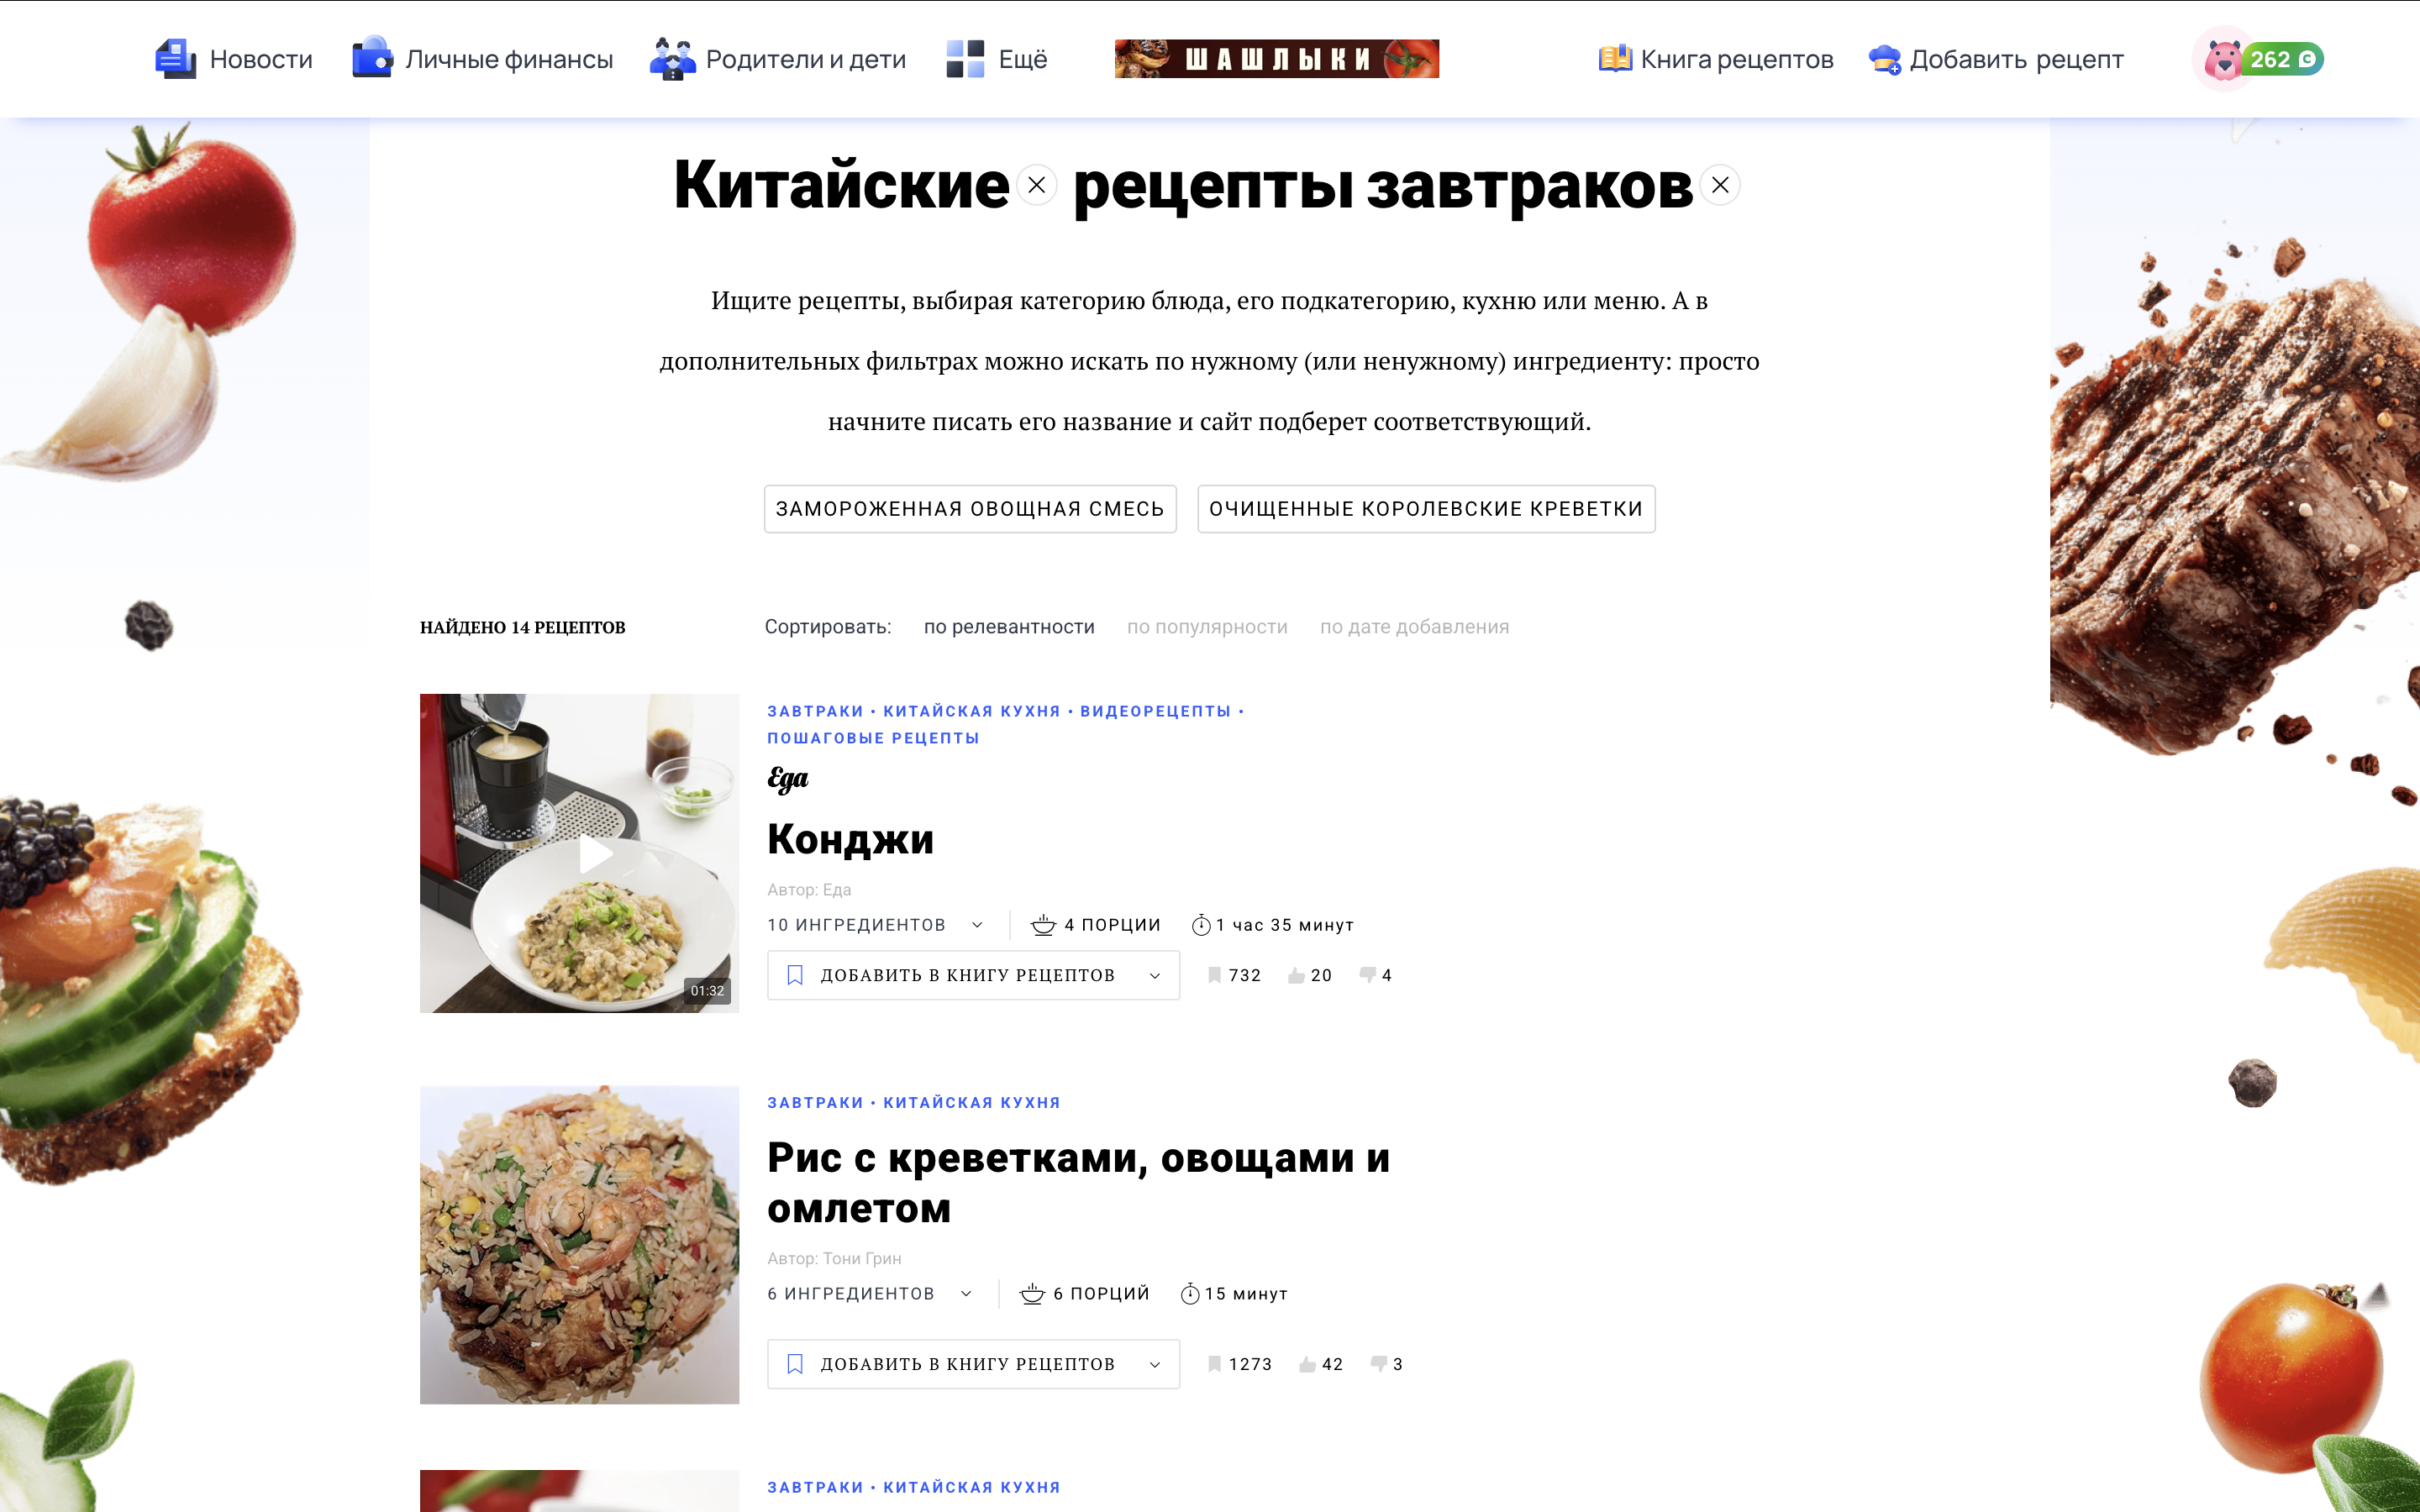
\includegraphics[width=\textwidth,height=0.82\textheight,keepaspectratio]{images/competitor-eda-rambler.png}
  }{
    \fbox{\parbox{0.92\textwidth}{\centering Файл скриншота не найден: \texttt{images/competitor-eda-rambler.png}}}
  }
  \caption{Интерфейс платформы Еда (Rambler)}
  \label{fig:competitor-eda-rambler}
\end{figure}

Ovkuse \cite{ovkuse2026} интересен сочетанием активного сообщества, большой базы рецептов и наличием ИИ-ассистента для быстрого подбора блюд. Сервис также предлагает расширенные сценарии просмотра и дополнительные блоки данных по рациону, что может быть полезно для вовлеченных пользователей. При этом значимая часть практической функциональности для регулярного использования переведена в подписочную модель, что снижает доступность для части аудитории. Кроме того, в платформе отсутствует полнофункциональный конструктор длительного плана питания в формате, необходимом для FoodPlanner. Интерфейс платформы Ovkuse представлен на рисунке~\ref{fig:competitor-ovkuse}.

\begin{figure}[H]
  \centering
  \IfFileExists{images/competitor-ovkuse.png}{
    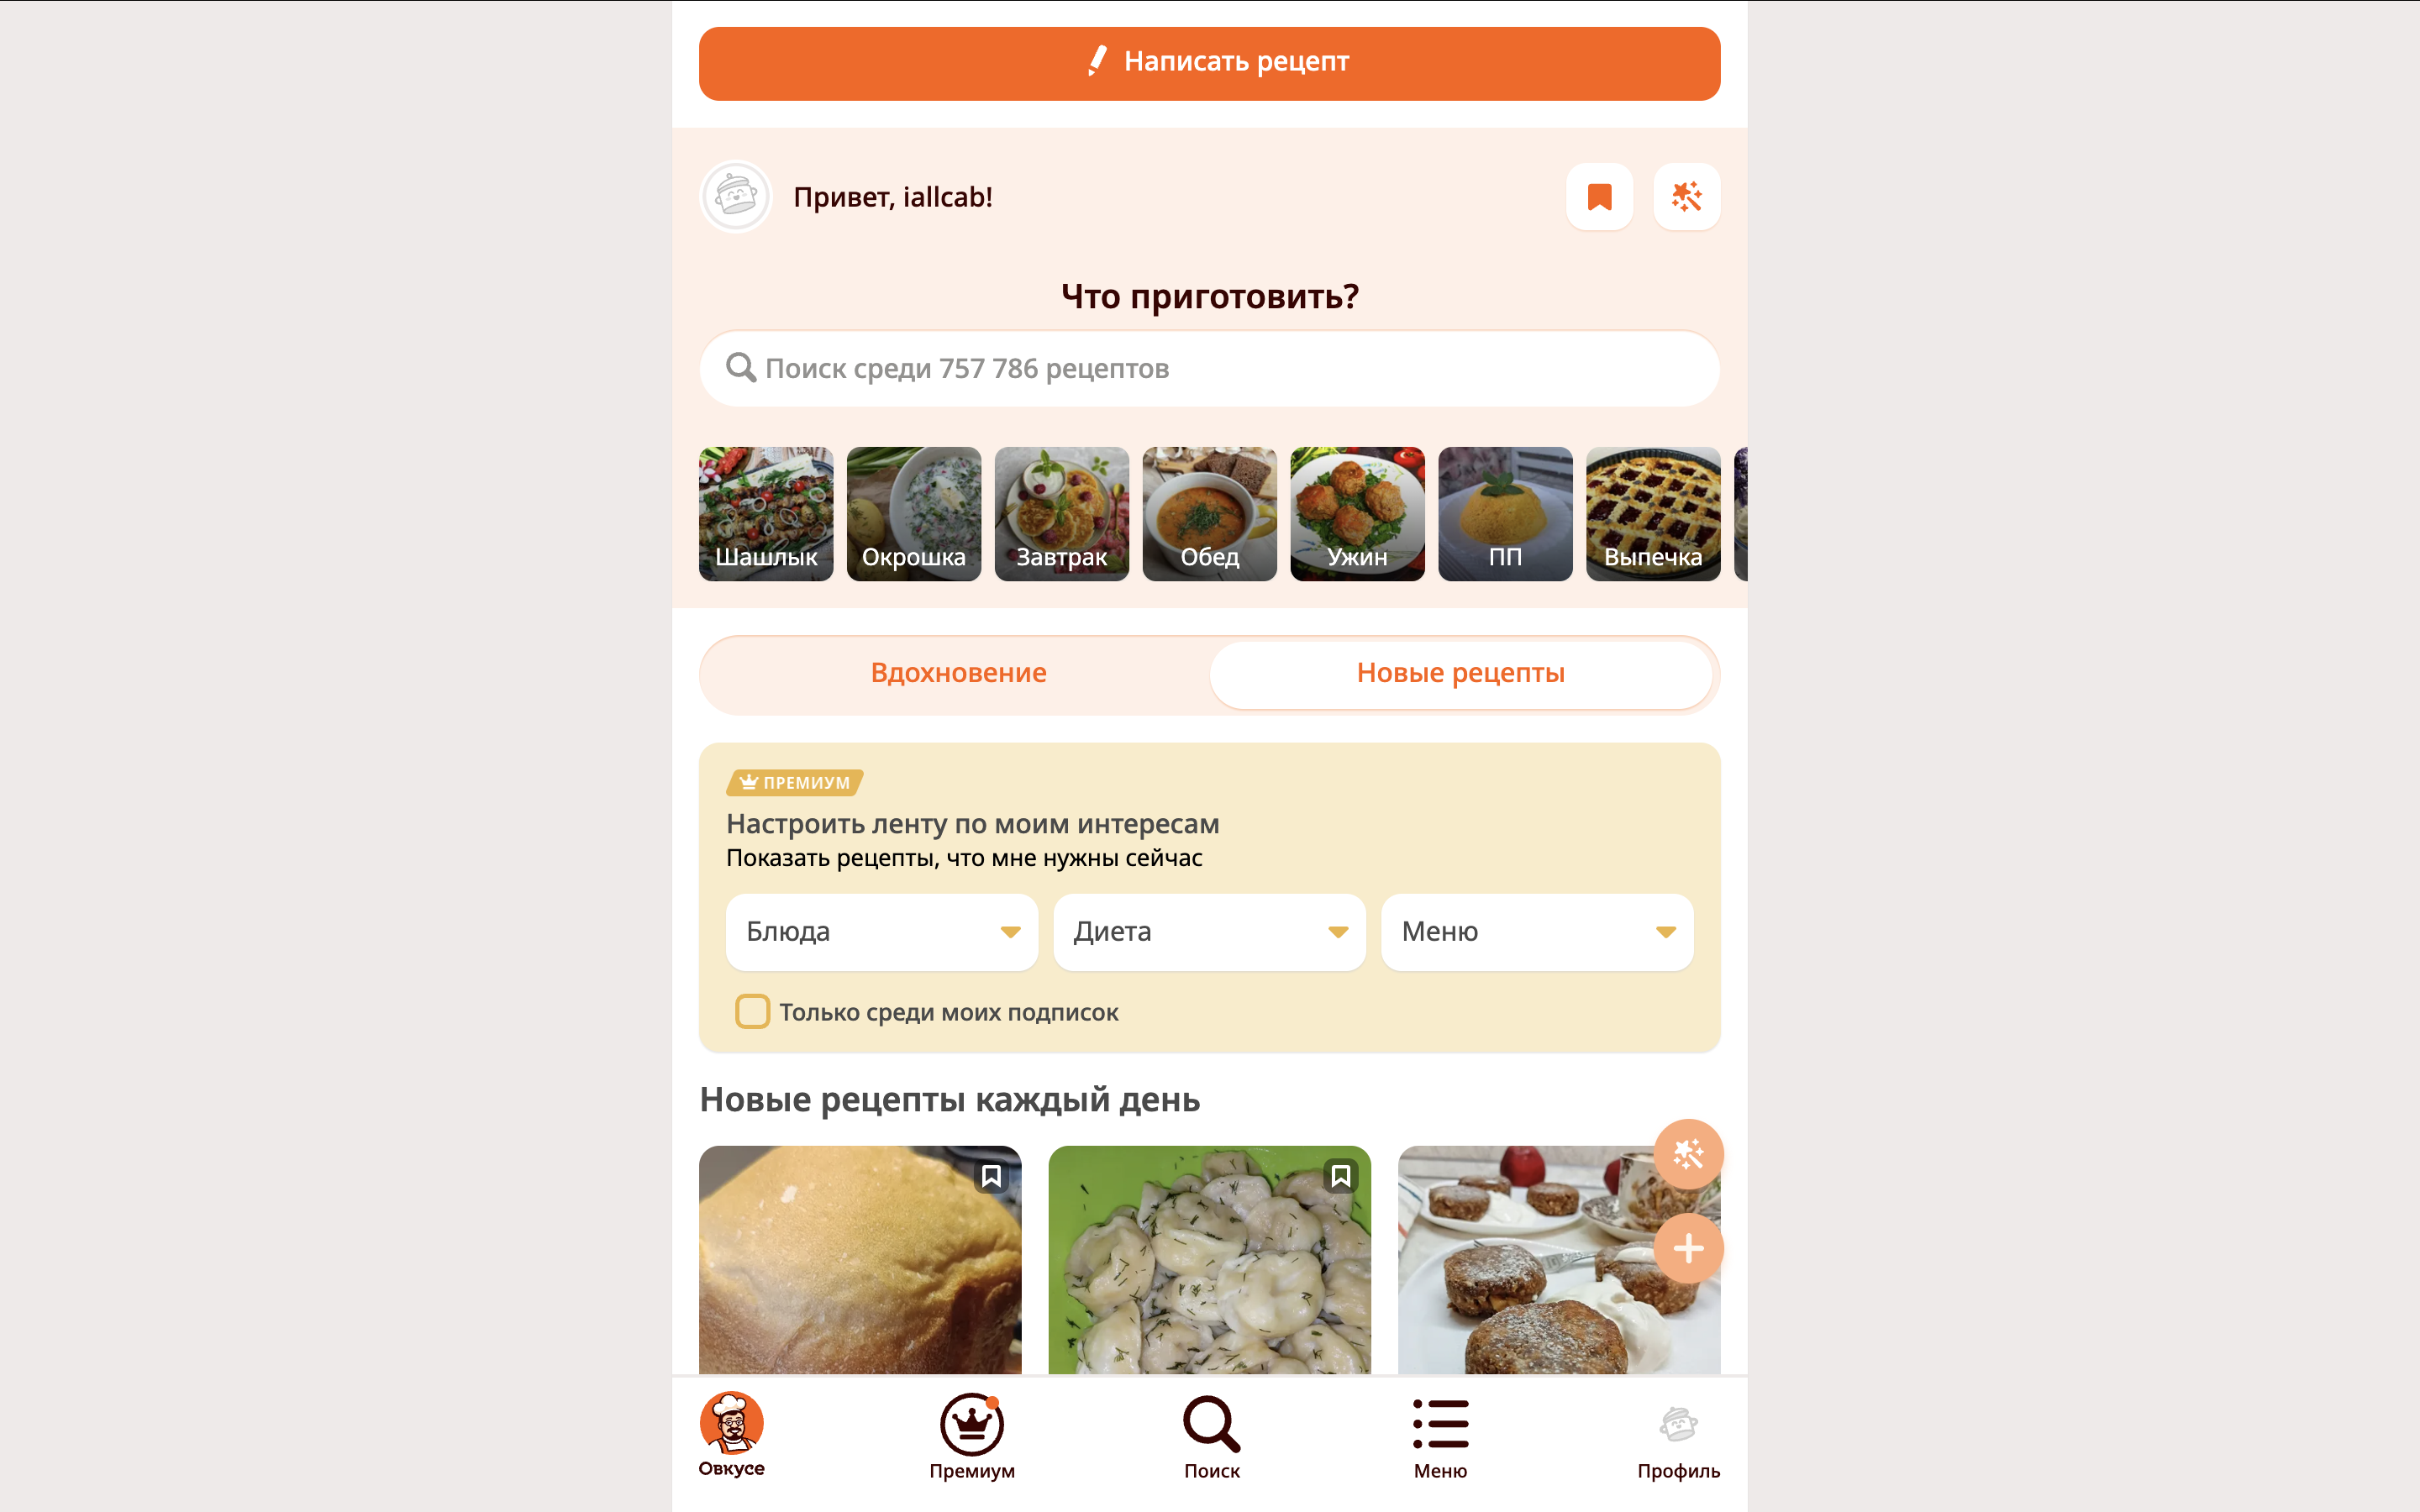
\includegraphics[width=\textwidth,height=0.82\textheight,keepaspectratio]{images/competitor-ovkuse.png}
  }{
    \fbox{\parbox{0.92\textwidth}{\centering Файл скриншота не найден: \texttt{images/competitor-ovkuse.png}}}
  }
  \caption{Интерфейс платформы Ovkuse}
  \label{fig:competitor-ovkuse}
\end{figure}

<<Поварёнок>> \cite{povarenok2026} остается сильным конкурентом как крупная кулинарная социальная платформа: в системе представлены рецепты, дневники пользователей, вопросы-ответы, статьи, посты и видеоконтент. Такой формат обеспечивает высокую активность сообщества и большой объем пользовательского контента. Одновременно интерфейс сервиса воспринимается как менее современный по сравнению с новыми продуктами, а ключевые функции FoodPlanner (конструктор плана питания и ИИ-помощник) не реализованы. Интерфейс платформы <<Поварёнок>> представлен на рисунке~\ref{fig:competitor-povarenok}.

\begin{figure}[H]
  \centering
  \IfFileExists{images/competitor-povarenok.png}{
    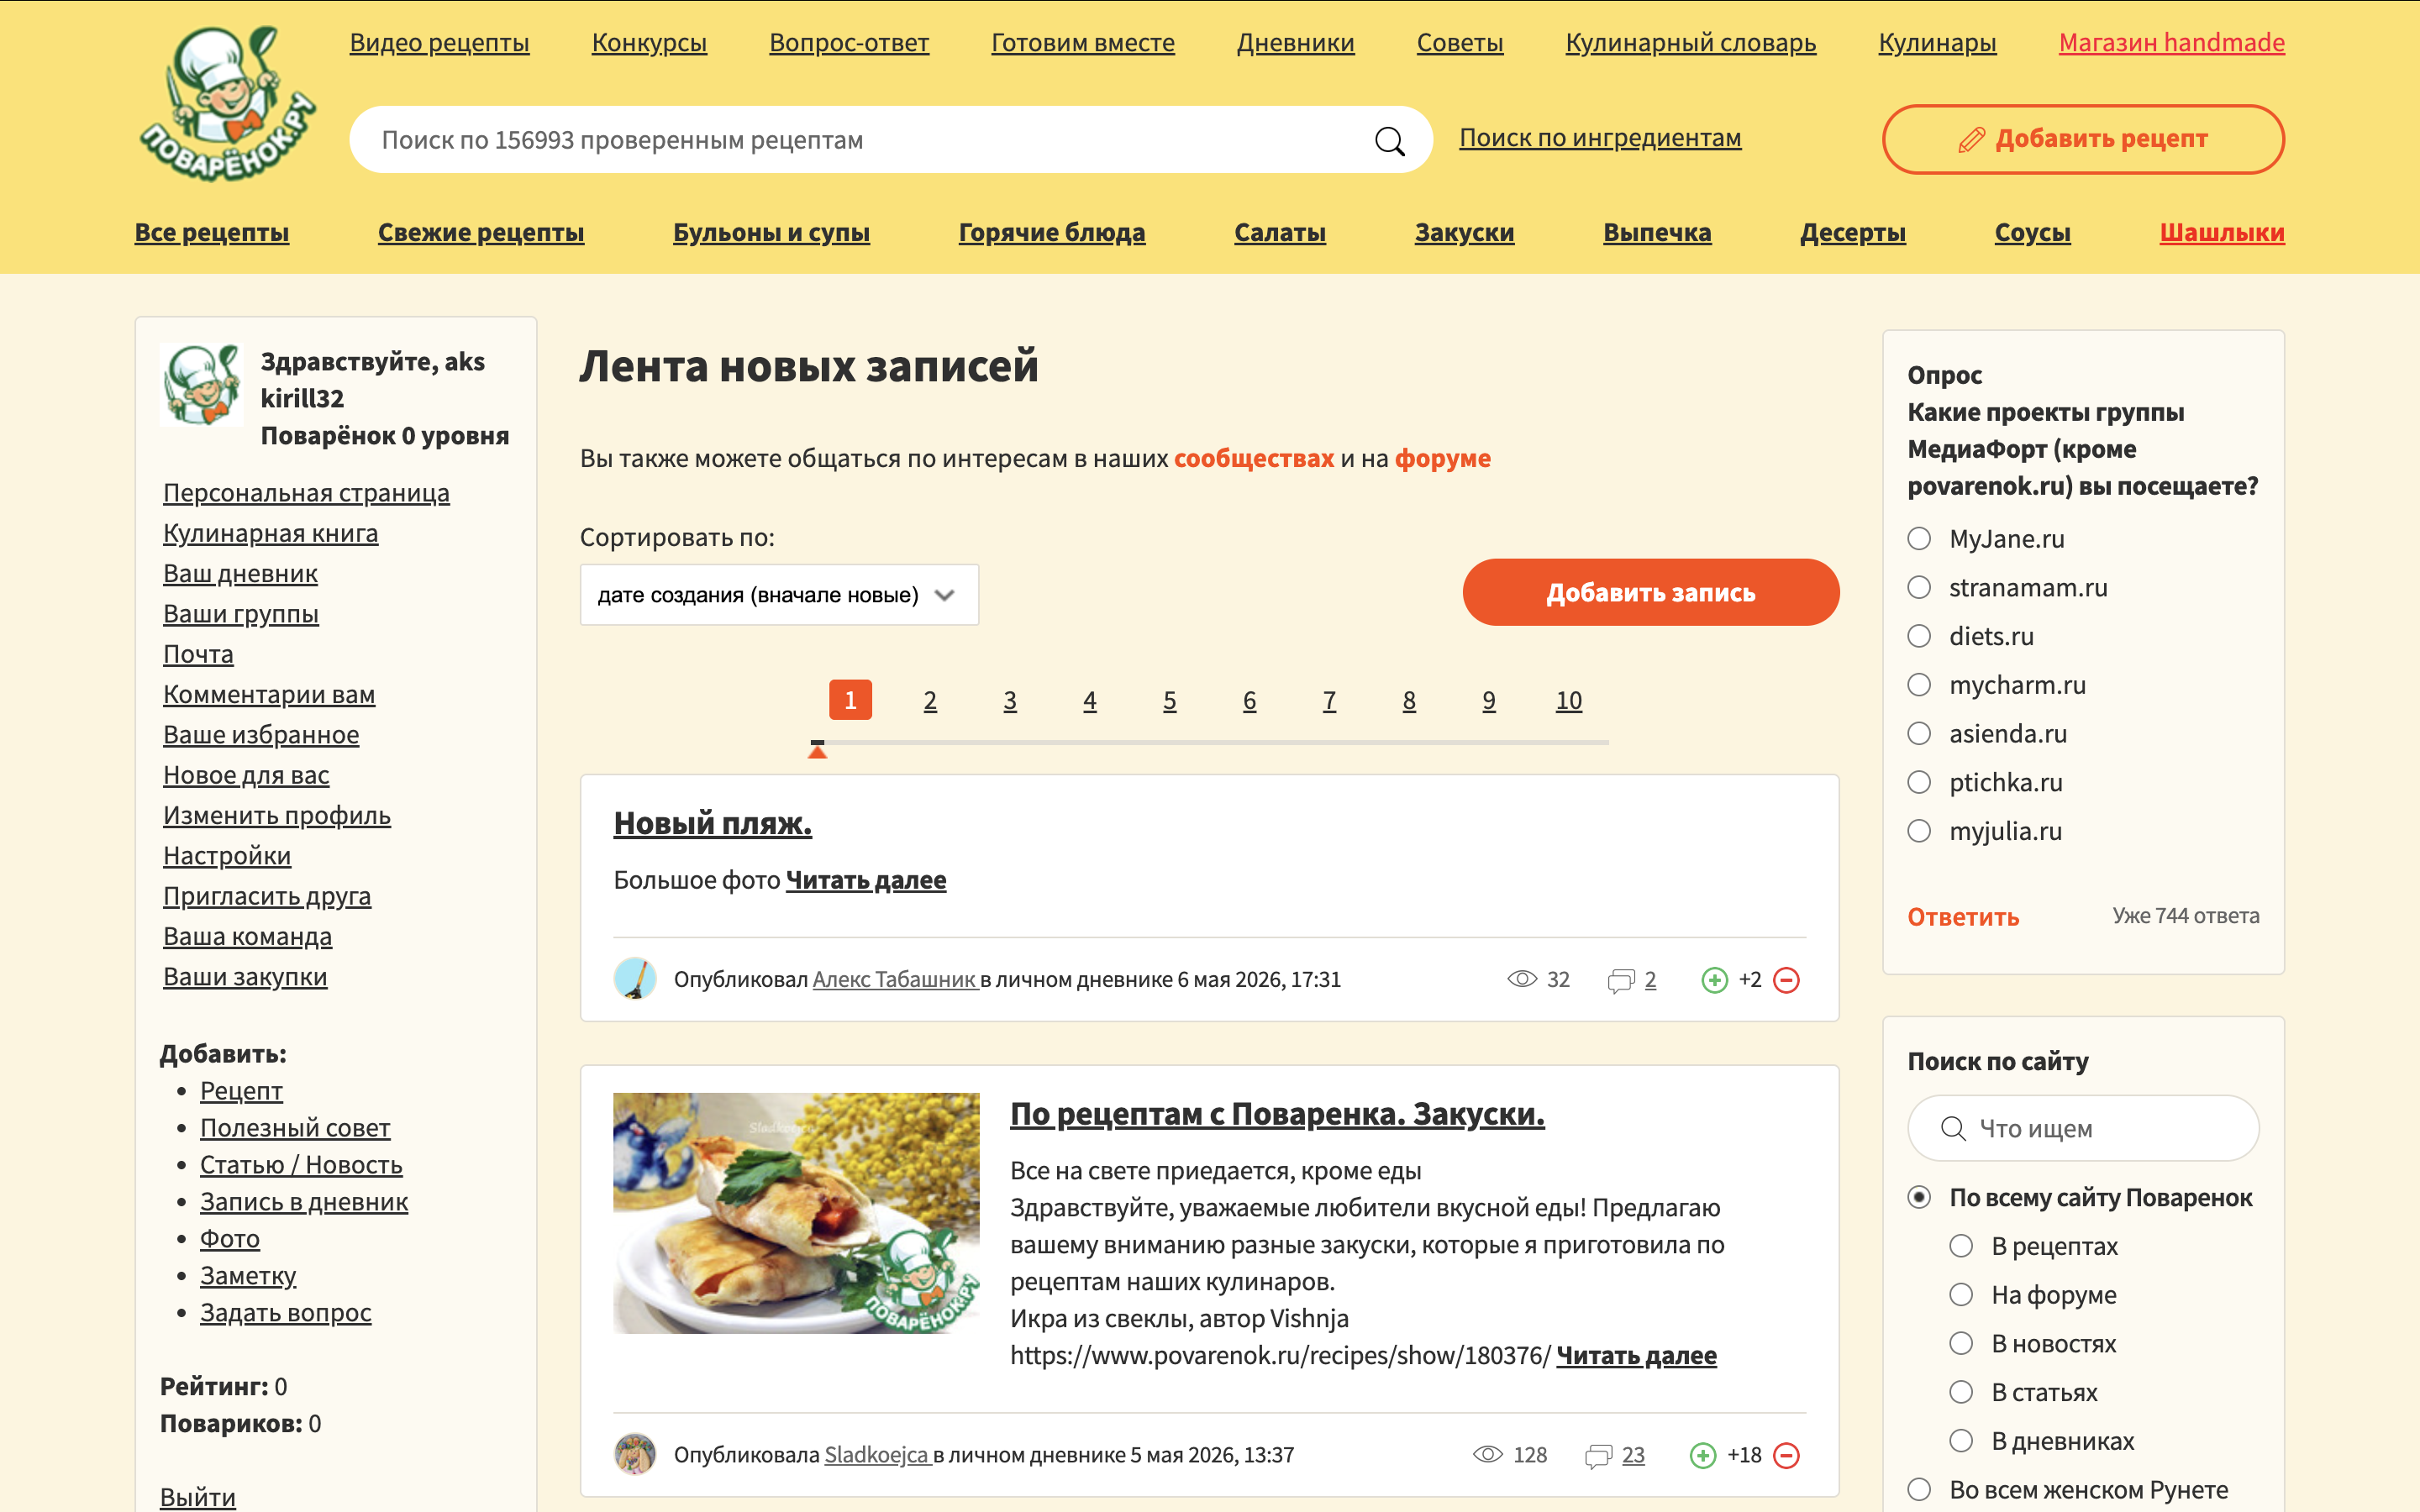
\includegraphics[width=\textwidth,height=0.82\textheight,keepaspectratio]{images/competitor-povarenok.png}
  }{
    \fbox{\parbox{0.92\textwidth}{\centering Файл скриншота не найден: \texttt{images/competitor-povarenok.png}}}
  }
  \caption{Интерфейс платформы Поварёнок}
  \label{fig:competitor-povarenok}
\end{figure}

MyFitnessPal \cite{myfitnesspal2026} задает высокий стандарт в области постановки целей и трекинга прогресса: при регистрации пользователю предлагается уточнить цель, мотивацию и параметры достижения, после чего доступны дневник питания и аналитические дэшборды. Платформа особенно сильна в фитнес- и weight-management сценариях, где важна регулярная фиксация показателей и динамики. Однако сервис в меньшей степени ориентирован на детализированное конструирование меню по дням и приемам пищи, а встроенный ИИ-ассистент отсутствует. Интерфейс платформы MyFitnessPal представлен на рисунке~\ref{fig:competitor-myfitnesspal}.

\begin{figure}[H]
  \centering
  \IfFileExists{images/competitor-myfitnesspal.png}{
    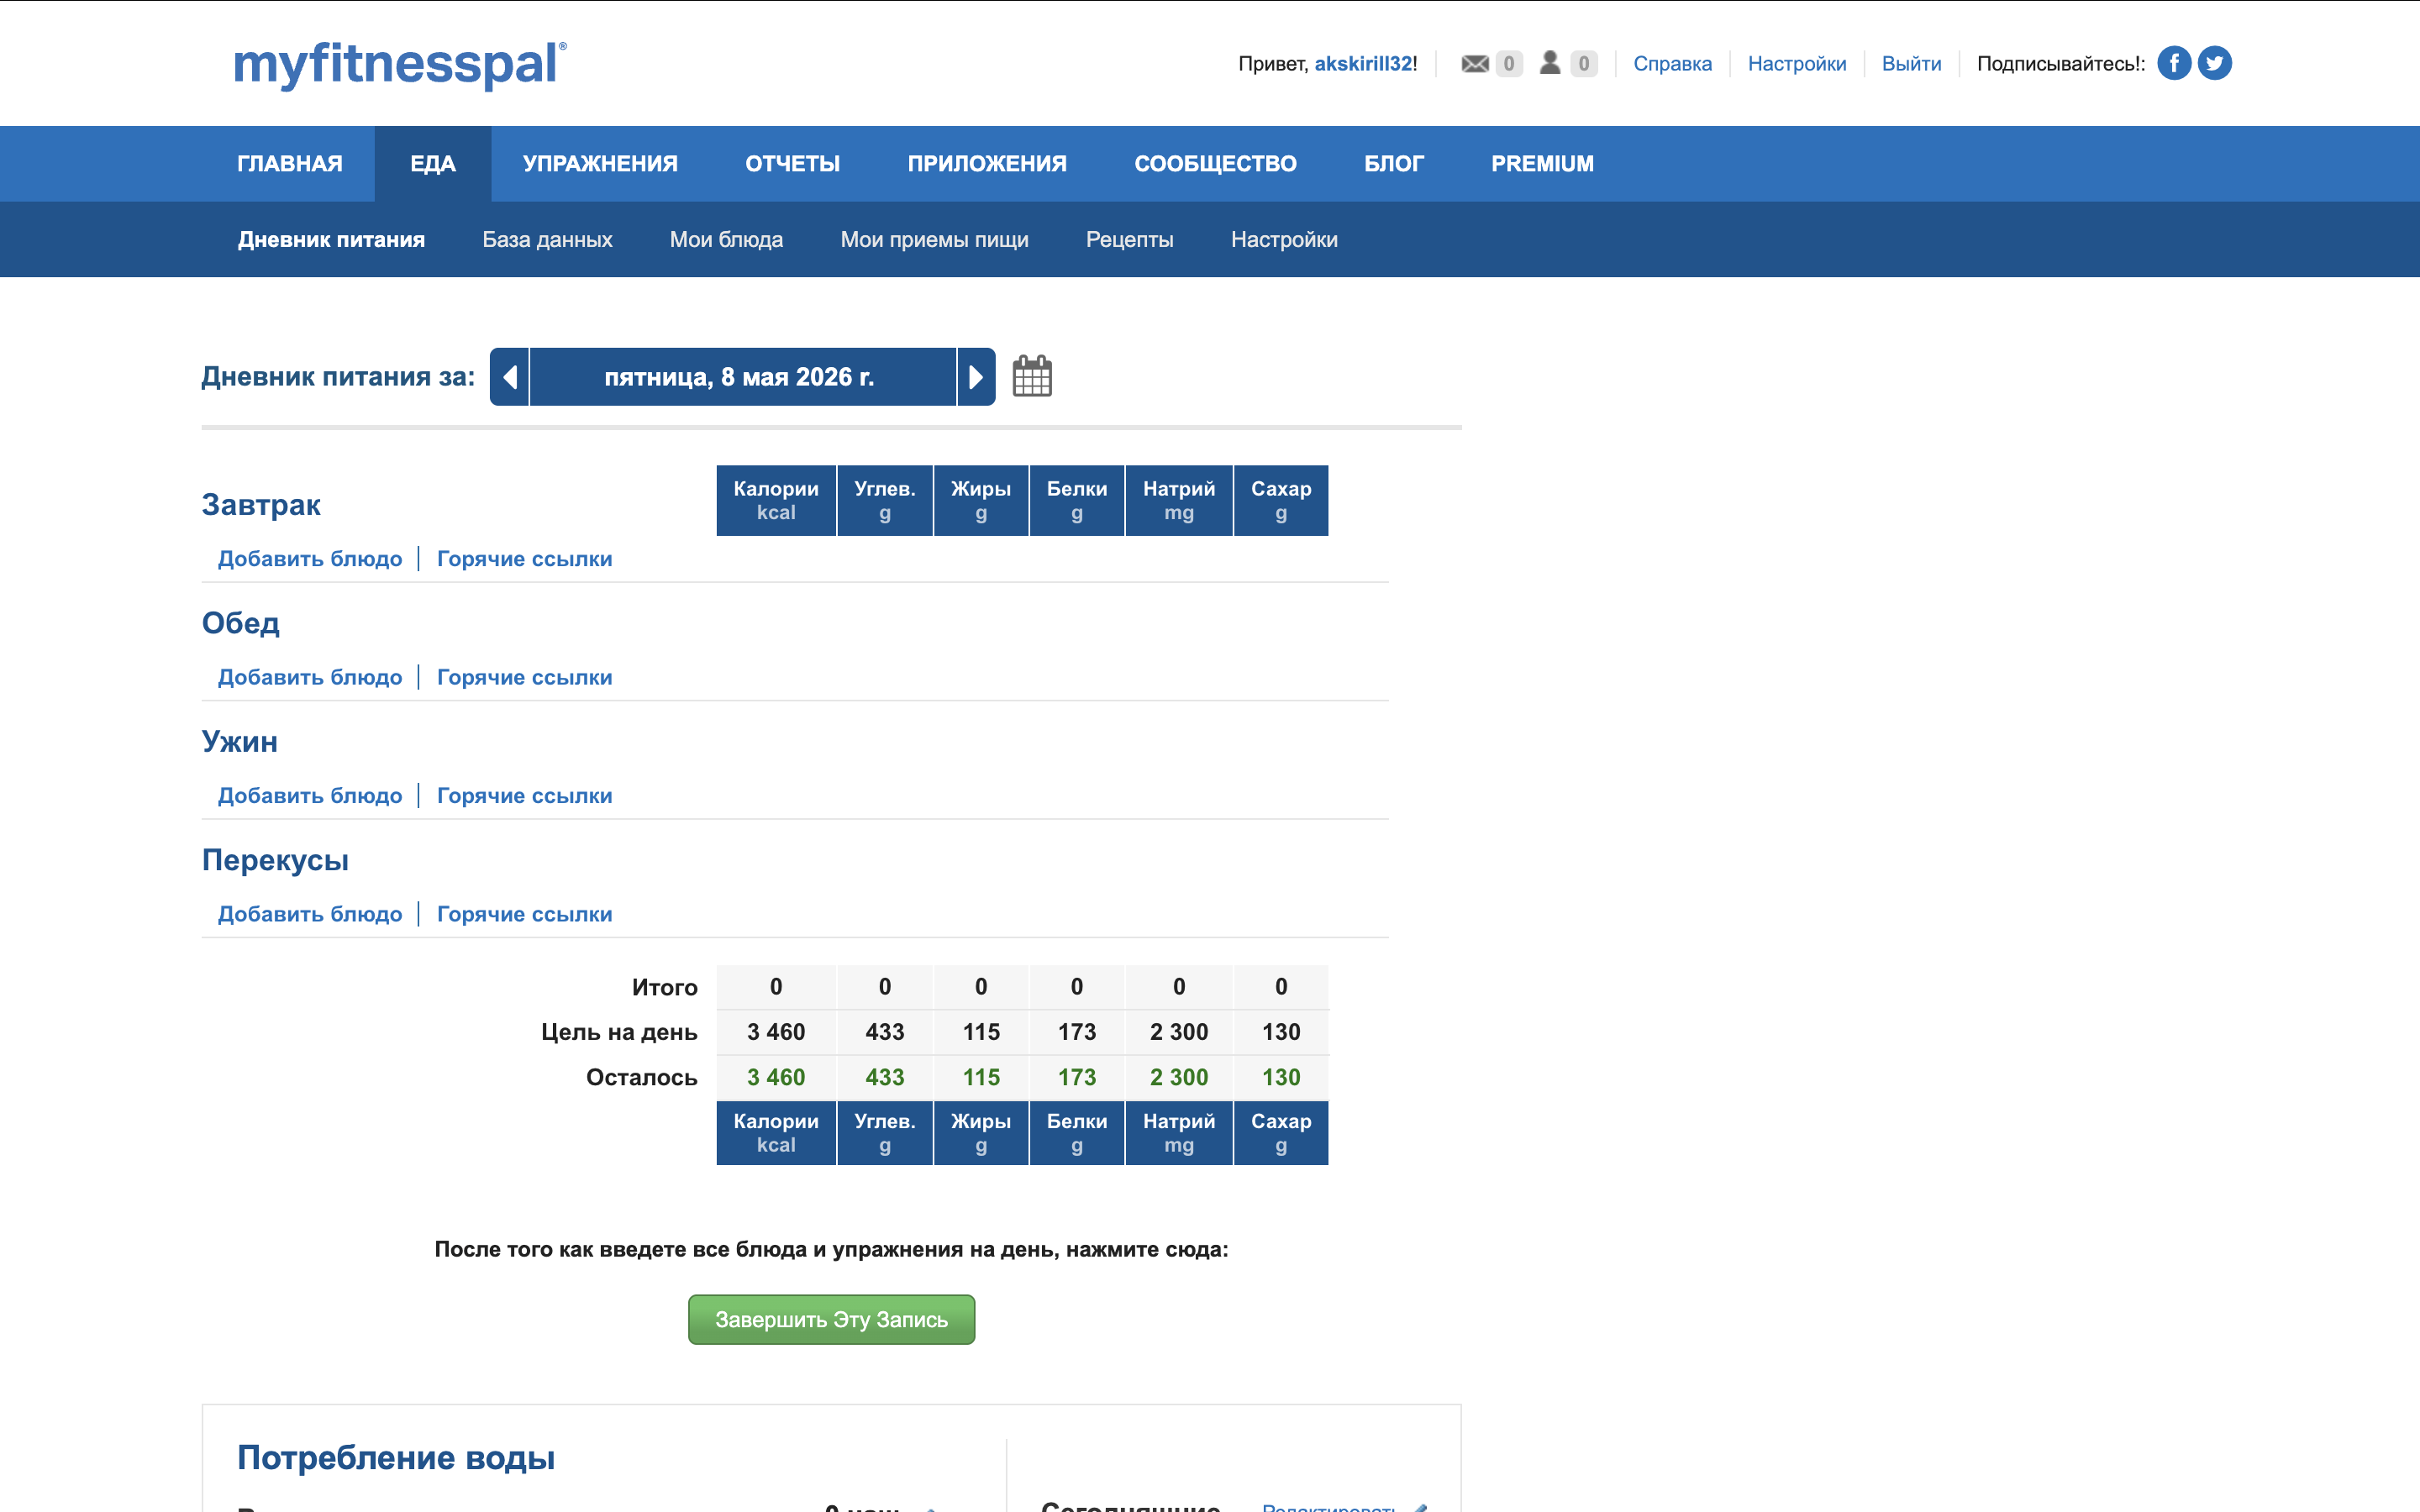
\includegraphics[width=\textwidth,height=0.82\textheight,keepaspectratio]{images/competitor-myfitnesspal.png}
  }{
    \fbox{\parbox{0.92\textwidth}{\centering Файл скриншота не найден: \texttt{images/competitor-myfitnesspal.png}}}
  }
  \caption{Интерфейс платформы MyFitnessPal}
  \label{fig:competitor-myfitnesspal}
\end{figure}

Проведенный анализ показывает, что конкуренты хорошо закрывают отдельные сегменты: контент и рецептуры, учет КБЖУ, мотивацию, социальные механики или частичную автоматизацию. При этом ни одно из рассмотренных решений не объединяет в едином контуре все целевые функции FoodPlanner: персонализированный конструктор плана питания, адаптацию под предпочтения пользователя, ИИ-сопровождение, списки покупок и ролевую модерацию контента.

\section{Определение требований к системе}

В данном разделе требования к системе представлены в порядке бизнес-приоритета: бизнес-требования, бизнес-правила и функциональные требования.

Бизнес-требования

Бизнес-требования сформулированы в измеримом виде (базовое значение~$\rightarrow$~целевое значение за 6 месяцев после запуска):
\begin{compactlist}
  \item удержание пользователей D30: 18\%~$\rightarrow$~30\%;
  \item конверсия из просмотра каталога в создание плана питания: 12\%~$\rightarrow$~25\%;
  \item доля пользователей, формирующих список покупок после создания плана: 20\%~$\rightarrow$~40\%;
  \item среднее время модерации пользовательского контента: 72~ч~$\rightarrow$~24~ч;
  \item доля жалоб, обработанных в пределах SLA 48~ч: 60\%~$\rightarrow$~90\%;
  \item доля контента с прозрачным отображением статуса модерации: 70\%~$\rightarrow$~100\%.
\end{compactlist}

Бизнес-правила

Бизнес-правила задают обязательные ограничения на поведение системы:
\begin{compactlist}
  \item ролевая модель обязательна: действия модерации доступны только ролям moderator и admin;
  \item жизненный цикл пользовательского контента фиксирован: \texttt{draft~$\rightarrow$~pending~$\rightarrow$~approved/rejected};
  \item пользователь может редактировать и удалять только собственный контент; администратор имеет расширенные права;
  \item при заполненном профиле предпочтений система обязана учитывать его в персонализированной выдаче;
  \item список покупок сохраняется с привязкой к источнику (рецепт или план питания) и доступен для повторного использования;
  \item изменения статусов модерации и ответы по жалобам сопровождаются созданием уведомлений;
  \item ключевые действия в процессах модерации и администрирования подлежат журналированию в аудите.
\end{compactlist}

Функциональные требования

Для реализации бизнес-целей выделены ключевые подсистемы, представленные в таблице~\ref{tab:subsystems-fp}.

\begin{table}[H]
\caption{Ключевые подсистемы FoodPlanner для реализации функциональных требований}
\label{tab:subsystems-fp}
\small
\begin{tabularx}{\textwidth}{|p{0.30\textwidth}|X|}
\hline
\multicolumn{1}{|c|}{Название подсистемы} & \multicolumn{1}{c|}{Описание} \\ \hline
Система управления аккаунтами и доступом & Регистрация, авторизация, управление профилем и ролевым доступом. \\ \hline
Система каталога и персонализации & Просмотр рецептов и планов, поиск, фильтрация и персонализированная выдача. \\ \hline
Система конструктора плана питания & Формирование меню по дням и приемам пищи, настройка параметров, отправка на модерацию. \\ \hline
Система модерации и обратной связи & Модерация рецептов, планов и отзывов, обработка жалоб, фиксация решений. \\ \hline
Система избранного и списков покупок & Сохранение рецептов/планов в избранное, формирование и хранение списков покупок. \\ \hline
Система уведомлений и ИИ-ассистента & Уведомления о событиях платформы и диалоговый интерфейс рекомендаций. \\ \hline
\end{tabularx}
\normalsize
\end{table}

На основании указанных подсистем сформулированы следующие функциональные требования:
\begin{compactlist}
  \item пользователь может зарегистрироваться в системе и выполнить вход по учетным данным;
  \item пользователь может просматривать и редактировать профиль (имя, фото, цели, особенности питания, теги);
  \item система поддерживает ролевую модель \texttt{user/moderator/admin} с разграничением прав;
  \item пользователь может просматривать каталоги рецептов и планов питания с поиском, фильтрацией и пагинацией;
  \item пользователь может создавать план питания в конструкторе и отправлять его на модерацию;
  \item модератор/администратор может принимать решения по модерации контента;
  \item пользователь может оставлять оценки и отзывы для рецептов и планов питания;
  \item пользователь может формировать и сохранять списки покупок с привязкой к рецепту или плану;
  \item система отображает уведомления о результатах операций и статусах модерации;
  \item пользователь может получать рекомендации через встроенный ИИ-ассистент.
\end{compactlist}

Нефункциональные требования

Ключевые нефункциональные требования:
\begin{compactlist}
  \item доступность сервиса в production: не ниже 99.5\% в месяц;
  \item медианное время ответа API для типовых запросов каталога: не более 500~мс;
  \item время загрузки ключевых страниц интерфейса при стандартном канале: не более 2~с;
  \item масштабируемость базы данных и API при росте объема данных не менее чем в 10 раз;
  \item безопасность: CSRF, ограничение CORS, хэширование паролей, HTTPS, отсутствие ключей внешних API на клиенте \cite{owasp_top10_2021,owasp_csrf_cheatsheet,owasp_xss_cheatsheet,owasp_sqli_cheatsheet,django_cors_headers_docs_2026};
  \item сопровождаемость: модульная структура frontend/backend и документированные контракты API.
\end{compactlist}

\section{Проектирование архитектуры системы}

Общая структура данных в приложении

Общая структура данных и потоков в FoodPlanner может быть формализована через DFD-представление. Контекстная диаграмма отражает взаимодействие системы с ключевыми внешними сущностями:
\begin{compactlist}
  \item пользователь платформы (формирование рациона, работа с рецептами и планами);
  \item модератор и администратор (контроль качества контента и управление системой);
  \item клиентское веб-приложение (SPA), выступающее основным каналом пользовательского взаимодействия;
  \item внешние сервисы (например, API ИИ-ассистента).
\end{compactlist}

Контекстная DFD-диаграмма представлена на рисунке~\ref{fig:dfd-context}.

\begin{figure}[H]
  \centering
  \IfFileExists{images/dfd-context.png}{
    
\includegraphics[width=\textwidth,height=0.82\textheight,keepaspectratio]{dfd-context.png}
  }{
    \fbox{\parbox{0.9\textwidth}{\centering Место для контекстной DFD-диаграммы\\
    Файл: \texttt{Report/images/dfd-context.png}}}
  }
  \caption{Контекстная DFD-диаграмма FoodPlanner}
  \label{fig:dfd-context}
\end{figure}

При детализации DFD-уровня выделяются основные процессы и хранилища данных.

Процессы:
\begin{compactlist}
  \item управление пользователями и аутентификацией;
  \item управление рецептами, тегами, категориями и ингредиентами;
  \item управление планами питания и генерацией списков покупок;
  \item модерация пользовательского контента и обработка жалоб;
  \item управление отзывами, избранным и уведомлениями;
  \item взаимодействие с внешним API ИИ-ассистента.
\end{compactlist}

Хранилища данных:
\begin{compactlist}
  \item DS1: учетные записи, роли и настройки профилей пользователей;
  \item DS2: рецепты, планы питания, структура рационов и shopping list;
  \item DS3: отзывы, жалобы, модерационные журналы и уведомления.
\end{compactlist}

Детализированная DFD-диаграмма представлена на рисунке~\ref{fig:dfd-level1}.

\begin{figure}[H]
  \centering
  \IfFileExists{images/dfd-level1.png}{
    
\includegraphics[width=\textwidth,height=0.82\textheight,keepaspectratio]{dfd-level1.png}
  }{
    \fbox{\parbox{0.9\textwidth}{\centering Место для детализированной DFD-диаграммы\\
    Файл: \texttt{Report/images/dfd-level1.png}}}
  }
  \caption{DFD-диаграмма процессов и хранилищ данных FoodPlanner}
  \label{fig:dfd-level1}
\end{figure}

Такая организация данных и потоков обеспечивает целостность информации и упрощает масштабирование системы при росте количества пользователей и контента.

Выбор архитектуры веб-сервиса

Для FoodPlanner выбрана клиент-серверная архитектура: клиентская часть (React + TypeScript) и серверная часть (Django + DRF) реализованы как независимые модули с единым API-контрактом. Альтернативным вариантом могла быть микросервисная архитектура, однако для текущего масштаба проекта и размера команды она избыточна по операционной сложности.

Схематичное представление клиент-серверной архитектуры и микросервисного подхода показано на рисунках~\ref{fig:arch-client-server} и~\ref{fig:arch-microservices}.

\begin{figure}[H]
  \centering
  \IfFileExists{images/arch-client-server.png}{
    
\includegraphics[width=\textwidth,height=0.82\textheight,keepaspectratio]{arch-client-server.png}
  }{
    \fbox{\parbox{0.9\textwidth}{\centering Место для схемы клиент-серверной архитектуры\\
    Файл: \texttt{Report/images/arch-client-server.png}}}
  }
  \caption{Клиент-серверная архитектура FoodPlanner}
  \label{fig:arch-client-server}
\end{figure}

\begin{figure}[H]
  \centering
  \IfFileExists{images/arch-microservices.png}{
    
\includegraphics[width=\textwidth,height=0.82\textheight,keepaspectratio]{arch-microservices.png}
  }{
    \fbox{\parbox{0.9\textwidth}{\centering Место для схемы микросервисной архитектуры\\
    Файл: \texttt{Report/images/arch-microservices.png}}}
  }
  \caption{Микросервисная архитектура (альтернативный подход)}
  \label{fig:arch-microservices}
\end{figure}

Сравнительный анализ клиент-серверной и микросервисной архитектур приведен в таблице~\ref{tab:arch-compare}.

\begin{table}[H]
\caption{Сравнение клиент-серверной и микросервисной архитектур}
\label{tab:arch-compare}
\small
\begin{tabularx}{\textwidth}{|p{0.21\textwidth}|p{0.36\textwidth}|X|}
\hline
\multicolumn{1}{|c|}{Критерий} & \multicolumn{1}{c|}{Клиент-серверная архитектура} & \multicolumn{1}{c|}{Микросервисная архитектура} \\ \hline
Принцип & Единый централизованный backend для обслуживания клиентов & Набор автономных сервисов, каждый отвечает за свою предметную область \\ \hline
Компоненты & SPA-клиент, API-сервер, единая БД & Набор сервисов, API-шлюз, межсервисное взаимодействие, распределенные БД \\ \hline
Масштабируемость & Масштабирование преимущественно на уровне всего backend & Независимое масштабирование отдельных сервисов \\ \hline
Развертывание & Единый релизный контур и более простой процесс деплоя & Независимые релизы, более сложная инфраструктура CI/CD \\ \hline
Сложность разработки & Ниже, проще старт и сопровождение малой командой & Выше из-за распределенности и усложнения инфраструктуры \\ \hline
Надежность при сбоях & Критические сбои затрагивают сервис целиком & Сбой одного сервиса ограниченно влияет на систему в целом \\ \hline
Коммуникация & Централизованные HTTP-запросы к одному API & HTTP/gRPC + асинхронные шины и очереди \\ \hline
Тестирование & Проще сквозное тестирование & Требуется отдельно тестировать сервисы и интеграции \\ \hline
\end{tabularx}
\normalsize
\end{table}

Для текущих требований FoodPlanner, объема команды и ресурсов клиент-серверная архитектура обеспечивает оптимальный баланс между скоростью разработки и эксплуатационной устойчивостью, сохраняя возможность дальнейшего масштабирования.

Для дальнейшей детализации архитектуры используется C4-подход, разделяющий описание системы на уровни абстракции:
\begin{compactlist}
  \item Context --- система в окружении пользователей и внешних сервисов;
  \item Container --- клиент, backend, база данных и внешние интеграции;
  \item Component --- внутренние модули backend и frontend по доменным областям;
  \item Code --- уровень классов/модулей и программной реализации.
\end{compactlist}

Проектирование базы данных

При выборе модели хранения данных для FoodPlanner рассматривались основные типы баз данных:
\begin{compactlist}
  \item реляционные БД --- строгая схема, SQL, ACID-транзакции, высокая целостность;
  \item документо-ориентированные БД --- гибкая схема и высокая адаптивность форматов;
  \item key-value и колоночные БД --- высокая производительность в специализированных сценариях.
\end{compactlist}

Сравнительная характеристика моделей данных представлена в таблице~\ref{tab:db-model-compare}.

\begin{table}[H]
\caption{Сравнительная характеристика моделей баз данных}
\label{tab:db-model-compare}
\small
\begin{tabularx}{\textwidth}{|p{0.22\textwidth}|p{0.24\textwidth}|X|}
\hline
\multicolumn{1}{|c|}{Критерий} & \multicolumn{1}{c|}{Реляционная модель} & \multicolumn{1}{c|}{Гибкие NoSQL-модели} \\ \hline
Структура данных & Таблицы, связи, строгая схема & Документы/ключ-значение/колонки, схема гибкая \\ \hline
Целостность & Высокая за счет ограничений и внешних ключей & Часто контролируется на уровне приложения \\ \hline
Транзакционность & Полная поддержка ACID & Поддержка зависит от конкретной СУБД \\ \hline
Язык запросов & Стандартизированный SQL & Специфичные API и языки запросов \\ \hline
Оптимальный сценарий & Бизнес-системы с богатой связностью данных и требованиями целостности & Высоконагруженные узкоспециализированные сценарии \\ \hline
\end{tabularx}
\normalsize
\end{table}

Для FoodPlanner выбрана реляционная модель с использованием PostgreSQL, так как система оперирует связанной доменной моделью (пользователи, рецепты, планы, отзывы, жалобы, уведомления), для которой критичны целостность, предсказуемость запросов и транзакционная согласованность.

Логическая схема данных отражает ключевые сущности предметной области и связи между ними. Центральными таблицами являются \texttt{users}, \texttt{recipes}, \texttt{ingredients}, \texttt{meal\_plans}, \texttt{reviews}, \texttt{complaints}, \texttt{favorites}, \texttt{notifications}, а также связующие таблицы \texttt{recipe\_ingredients}, \texttt{meal\_plan\_items}, \texttt{shopping\_list\_items}.

Внешние ключи, ограничения уникальности и индексы обеспечивают корректность и производительность типовых пользовательских запросов.

Ключевые элементы логической модели представлены ниже фрагментами реальной серверной реализации.

\begin{listing}[H]
\caption{Модель ролей и пользователей}
\label{listing:user-role-model}
\begin{mdframed}
\begin{minted}[breaklines=true]{python}
class Role(models.Model):
    class RoleNames(models.TextChoices):
        USER = "user", "User"
        MODERATOR = "moderator", "Moderator"
        ADMIN = "admin", "Admin"

    name = models.CharField(max_length=32, unique=True, choices=RoleNames.choices)

class User(AbstractUser):
    username = None
    email = models.EmailField(unique=True)
    role = models.ForeignKey(Role, on_delete=models.SET_NULL, null=True, blank=True)
    health_features = models.JSONField(default=list, blank=True)
    favorite_tags = models.JSONField(default=list, blank=True)
    USERNAME_FIELD = "email"
\end{minted}
\end{mdframed}
\end{listing}

\begin{listing}[H]
\caption{Фрагмент модели рецептов и состава ингредиентов}
\label{listing:recipe-model}
\begin{mdframed}
\begin{minted}[breaklines=true]{python}
class Recipe(models.Model):
    title = models.CharField(max_length=255)
    category = models.ForeignKey(Category, on_delete=models.SET_NULL, null=True, blank=True)
    author = models.ForeignKey(settings.AUTH_USER_MODEL, on_delete=models.CASCADE)
    status = models.CharField(max_length=16, choices=ModerationStatus.choices)
    tags = models.ManyToManyField(Tag, related_name="recipes", blank=True)

    class Meta:
        indexes = [
            models.Index(fields=["author"]),
            models.Index(fields=["category"]),
            models.Index(fields=["status"]),
        ]

class RecipeIngredient(models.Model):
    recipe = models.ForeignKey(Recipe, on_delete=models.CASCADE, related_name="recipe_ingredients")
    ingredient = models.ForeignKey(Ingredient, on_delete=models.CASCADE)
    quantity = models.DecimalField(max_digits=10, decimal_places=2)
\end{minted}
\end{mdframed}
\end{listing}

\begin{listing}[H]
\caption{Фрагмент модели плана питания и списка покупок}
\label{listing:mealplan-shopping-model}
\begin{mdframed}
\begin{minted}[breaklines=true]{python}
class MealPlan(models.Model):
    user = models.ForeignKey(settings.AUTH_USER_MODEL, on_delete=models.CASCADE)
    start_date = models.DateField()
    end_date = models.DateField()
    status = models.CharField(max_length=16, choices=Status.choices, default=Status.DRAFT)

class MealPlanItem(models.Model):
    meal_plan = models.ForeignKey(MealPlan, on_delete=models.CASCADE, related_name="items")
    day_number = models.PositiveSmallIntegerField()
    meal_type = models.CharField(max_length=16, choices=MealType.choices)
    recipe = models.ForeignKey("recipes.Recipe", on_delete=models.CASCADE)

class ShoppingList(models.Model):
    user = models.ForeignKey(settings.AUTH_USER_MODEL, on_delete=models.CASCADE)
    target_type = models.CharField(max_length=16, choices=TargetType.choices, blank=True, default="")
    target_id = models.PositiveBigIntegerField(null=True, blank=True)
\end{minted}
\end{mdframed}
\end{listing}

\begin{figure}[H]
  \centering
  \IfFileExists{images/data-model.png}{
    
\includegraphics[width=0.95\textwidth]{data-model.png}
  }{
    \fbox{\parbox{0.9\textwidth}{\centering Место для ER-диаграммы\\
    Файл: \texttt{Report/images/data-model.png}}}
  }
  \caption{Логическая модель данных FoodPlanner}
  \label{fig:data-model}
\end{figure}

\section{Выбор программных и технических средств разработки}

Для разработки FoodPlanner использован клиент-серверный подход, поэтому технологический стек разделен на две части: клиентскую (frontend) и серверную (backend). При выборе инструментов учитывались критерии производительности, скорости разработки, удобства сопровождения, зрелости экосистемы и соответствия функциональным требованиям проекта.

Серверная часть реализована на Python с использованием Django и Django REST Framework \cite{python_docs_2026,django_docs_2026,drf_docs_2026}. В качестве СУБД выбрана PostgreSQL \cite{postgresql_docs_2026}. Для контейнеризации и воспроизводимого развертывания используется Docker и Docker Compose \cite{docker_docs_2026,docker_compose_docs_2026}.

Для клиентской части выбраны React + TypeScript, управление состоянием выполнено на Effector, UI-слой построен на Mantine, сборка и локальная разработка выполняются через Vite \cite{react_docs_2026,typescript_docs_2026,effector_docs_2026,mantine_docs_2026,vite_docs_2026}.

Сравнительный анализ серверных языков разработки для проекта приведен в таблице~\ref{tab:backend-lang-compare} с опорой на официальные материалы по языкам и платформам \cite{python_docs_2026,java_docs_2026,nodejs_docs_2026,go_docs_2026}.

\begin{table}[H]
\caption{Сравнительный анализ серверных языков}
\label{tab:backend-lang-compare}
\begin{tabularx}{\textwidth}{|p{0.16\textwidth}|p{0.38\textwidth}|X|}
\hline
\multicolumn{1}{|c|}{Язык} & \multicolumn{1}{c|}{Преимущества} & \multicolumn{1}{c|}{Ограничения для проекта} \\ \hline
Python & Высокая скорость разработки, зрелые веб-фреймворки, низкий порог вхождения & Ниже производительность в CPU-интенсивных задачах по сравнению с компилируемыми языками \\ \hline
Java & Высокая надежность и производительность, зрелая экосистема enterprise-решений & Более высокая сложность и объем кода для быстрого прототипирования \\ \hline
Node.js (TS/JS) & Единый язык для frontend/backend, высокая скорость I/O-сценариев & Требует более строгой дисциплины архитектуры в больших проектах \\ \hline
Go & Высокая производительность и эффективная конкурентность & Меньшая гибкость и более узкая экосистема для сложных административных сценариев \\ \hline
\end{tabularx}
\end{table}

Для прикладных задач FoodPlanner (быстрая реализация доменных модулей, ролевой доступ, модерация, административная логика, API-подход) выбор Python + Django признан оптимальным по балансу трудозатрат и эксплуатационной надежности.

Сравнение выбранных средств клиентской разработки приведено в таблице~\ref{tab:frontend-stack-compare}.

\begin{table}[H]
\caption{Выбор средств клиентской разработки}
\label{tab:frontend-stack-compare}
\begin{tabularx}{\textwidth}{|p{0.26\textwidth}|X|}
\hline
\multicolumn{1}{|c|}{Компонент стека} & \multicolumn{1}{c|}{Обоснование выбора} \\ \hline
React + TypeScript & Компонентный подход, типобезопасность и удобная поддержка сложных интерфейсных сценариев \\ \hline
Effector & Детерминированное управление состоянием и понятная модель асинхронных процессов \\ \hline
Mantine & Быстрое построение консистентного UI и сокращение времени реализации типовых паттернов \\ \hline
Vite & Быстрый цикл разработки и сборки SPA-приложения \\ \hline
\end{tabularx}
\end{table}

Таким образом, выбранные программные и технические средства обеспечивают покрытие функциональных требований, поддержку безопасного взаимодействия клиентской и серверной частей, а также возможность поэтапного масштабирования системы.

\section{Выводы по главе}

В первой главе определен проблемный контекст предметной области: пользователи решают взаимосвязанные задачи планирования питания в разрозненных сервисах, что приводит к фрагментации данных и избыточным трудозатратам.

На основании обзора аналогов подтверждено наличие рыночных решений с сильными сторонами, однако выявлены ограничения при реализации комплексного сценария. Это обосновывает разработку собственного веб-приложения, объединяющего полный цикл планирования рациона.

Также сформированы целевая аудитория и ролевая модель, определены функциональные, бизнес- и нефункциональные требования, проведен сравнительный анализ конкурентов и аналогов, описаны бизнес-процессы в IDEF-нотациях и зафиксирована модель данных системы.